
\documentclass[letterpaper, 10 pt, conference]{ieeeconf}  
\IEEEoverridecommandlockouts\overrideIEEEmargins
% See the \addtolength command later in the file to balance the column lengths
% on the last page of the document

\usepackage{graphicx}
\usepackage{amsmath}
\usepackage{tikz}
\usepackage{circuitikz}
\usepackage{calc}
\usepackage{circuitikz}
\usetikzlibrary{calc}
\usepackage{multirow}
\usepackage[document]{ragged2e}

\title{\LARGE \bf
avr-gcc Assignment
}
\vspace{4mm}
\author{Naresh Gavvala \hspace{9cm} August 2022}


\begin{document}
\maketitle

\begin{abstract}
state any one Absorpion law of boolean algebra and verify it using truth table
\end{abstract}
\tableofcontents

\section{Components}\hfill\break
{
\centering
\begin{tabular}{|c|c|c|}
\hline
$\boldsymbol{Component}$&$\boldsymbol{Value}$&$\boldsymbol{Count}$\\
\hline
Arduino&UNO&1\\
\hline
\end{tabular}\par
}
\vspace{5mm} %5mm vertical space
\section{Absorption Law}
Absorptive Law – This law allows for the reduction of a difficult statement to a simpler one by absorbing phrases that are similar in structure. 
A + (A.B) = (A.1) + (A.B) = A(1 + B) = A (OR Absorption Law)
A(A + B) = (A + 0)
A(A + B) = A + (0.B) = A (AND Absorption Law)
A(A + B) =A

\vspace{1mm} %1mm vertical space
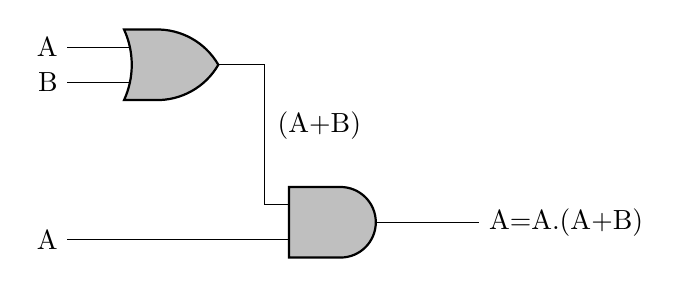
\begin{tikzpicture}
 
% Circuit style
\ctikzset{
    logic ports=ieee,
    logic ports/scale=0.8,
    logic ports/fill=lightgray
}
 
% Logic ports
\node[or port] (ORa) at (0,0){};
\node[and port] (ANDa) at (2,-2){};
 
 
% Connection
\draw (ORa.in 1) -- ++(-0.5,0)node[left](A){A};
\draw (ORa.in 2) -- ++(-0.5,0)node[left](B){B};
\draw (ANDa.in 2) -- ++(-2.5,0)node[left](A){A};

\draw (ORa.out) -| (ANDa.in 1) ++(0.7,0.7)node[above]{(A+B)};
\draw (ANDa.out) -- ++(1,0) node[right]{A=A.(A+B)};
 
\end{tikzpicture}\\
\vspace{1cm}
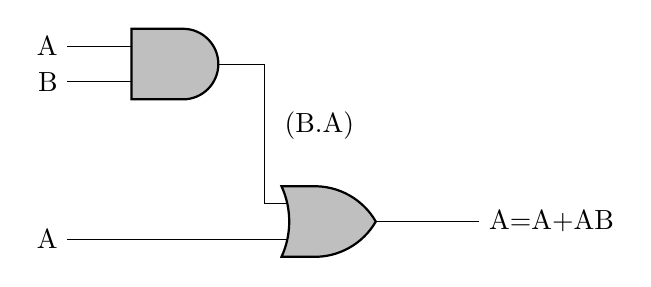
\begin{tikzpicture} 
% Circuit style
\ctikzset{
    logic ports=ieee,
    logic ports/scale=0.8,
    logic ports/fill=lightgray
}
 
% Logic ports
\node[and port] (ANDa) at (0,0){};
\node[or port] (ORa) at (2,-2){};
 
 
% Connection
\draw (ANDa.in 1) -- ++(-0.5,0)node[left](A){A};
\draw (ANDa.in 2) -- ++(-0.5,0)node[left](B){B};
\draw (ORa.in 2) -- ++(-2.5,0)node[left](A){A};

\draw (ANDa.out) -| (ORa.in 1) ++(0.7,0.7)node[above]{(B.A)};
\draw (ORa.out) -- ++(1,0) node[right]{A=A+AB};
 
\end{tikzpicture}\\
\vspace{10mm}


\subsection*{\normalsize Truth Table}
{
\[ A + A.B = A \]
\centering
\begin{tabular}{|c|c|c|c|}
\hline
${A}$&${B}$&${A.B}$&${(A+A.B)}$\\
\hline
0&0&0&0\\%
\hline
0&1&0&0\\%
\hline
1&0&0&1\\%
\hline
1&1&1&1\\%
\hline

\end{tabular}\par
}
\vspace{5mm} %5mm vertical space
\[A.(A + B) = A  \]
{
\centering
\begin{tabular}{|c|c|c|c|}
\hline
${A}$&${B}$&${A+B}$&${A.(A+B)}$\\
\hline
0&0&0&0\\%
\hline
0&1&1&0\\%
\hline
1&0&1&1\\%
\hline
1&1&1&1\\%
\hline
\end{tabular}\par
}
\vspace{5mm} %5mm vertical space
\section{Procedure:}
1) First make the 2,3,4,5 pins as output pins.
\\ 2)Write the given logic in code and upload in to the arduino.
\\ 5)The out put will be displayed in display either 1 or 0 corresponds to truth table.
\vspace{5mm} %5mm vertical space

\begin{enumerate}
\item svn co https://github.com/Ngavvala/fwc
\item cd ide\_assignment
\item pio run
\item pio run \--t upload

\end{enumerate}



\addtolength{\textheight}{-12cm}   % This command serves to balance the column lengths
                                  % on the last page of the document manually. It shortens
                                  % the textheight of the last page by a suitable amount.
                                  % This command does not take effect until the next page
                                  % so it should come on the page before the last. Make
                                  % sure that you do not shorten the textheight too much.

\end{document}
